%!TEX root = proj.tex

\section{Statistical analysis}
In the previous sections the two data sets have been presented, including descriptive statistics of each of them. Furthermore a normalized measure for travel demand deviations from the normal pattern, \gls{re_i}, has been modeled and checked. With this, the statistical analysis of the impact of weather on travel demand can be conducted.

\subsection{Merge of weather and travel demand}
Recall from \Cref{ch:desc_weather} that the weather time series have three time steps within each hour, while travel demand has only one measurement per hour. In order to merge the two data sets the weather time series is aggregated to the same granularity as described in \Cref{eq:temp_i,eq:pptn_i,eq:rh_i,eq:ws_i,eq:cond_i}.
\begin{align}
	\mathit{temp}_i &= \mathrm{mean}(\mathit{temp}_j, \mathit{temp}_{j + 1}, \mathit{temp}_{j + 2}) &\text{where} \; t_i = t_j 
	\label{eq:temp_i} \\
	\mathit{pptn}_i &= \mathrm{max}(\mathit{pptn}_j, \mathit{pptn}_{j + 1}, \mathit{pptn}_{j + 2}) &\text{where} \; t_i = t_j 
	\label{eq:pptn_i} \\
	\mathit{rh}_i &= \mathrm{max}(\mathit{rh}_j, \mathit{rh}_{j + 1}, \mathit{rh}_{j + 2}) &\text{where} \; t_i = t_j 
	\label{eq:rh_i} \\
	\mathit{ws}_i &= \mathrm{max}(\mathit{ws}_j, \mathit{ws}_{j + 1}, \mathit{ws}_{j + 2}) &\text{where} \; t_i = t_j
	\label{eq:ws_i} \\	
	\mathit{cond}_i &= \mathrm{max}(\mathit{cond}_j, \mathit{cond}_{j + 1}, \mathit{cond}_{j + 2}) &\text{where} \; t_i = t_j 
	\label{eq:cond_i}
\end{align}

\subsection{Univariate analysis}
Before going into the multivariate analysis, it is desirable to look for  of the correlations between the pairs of variables. \Cref{fig:cor_matrix} shows visualizes the correlation matrix of the numeric variables (e.g.\ without weather condition, \gls{cond_i}, day type, \gls{daytype_i}, and peek class, \gls{peek_i}). There are no clear linear correlations between pairs that surfaces, only a week correlation between wind speed, \gls{ws_i}, and \gls{re_i}, and a even more week correlation between temperature, \gls{temp_i}, and \gls{re_i}. 

The discrete variables (weather condition, \gls{cond_i}, day type, \gls{daytype_i}, and peek class, \gls{peek_i}) is investigated using ANOVA to test whether they contribute to \gls{re_i}. It is found with strong evidence ($F = 38.147$, $p < 0.001$) that the weather condition is influencing the travel demand, and the relationship is shown in \Cref{fig:cor_cond}. This is of cause not that surprising, and expected that rain impacts with an increased travel demand, but it is also possible to quantify the impact: E.g.\ heavy rain increases travel demand on average with over 12\%, while light rain and rain increases with approx. 3\% and 6\%. as shown in \Cref{tab:mean_cond_tab}. On the other hand is cannot been shown that day type, \gls{daytype_i}, and peek class, \gls{peek_i}, has influence ($F =  0.1395$, $p = 0.709$ respectable $F =  0.0463$, $p = 0.955$), i.e.\ the weather condition impacts similarly regardless of people are on their way to work or using public transport for leisure rides, which is interesting.
\begin{table}[!ht]
    \center
    \begin{tabular}{lr}
 $\mathit{cond}$ & Mean. $\mathit{re}_i$ \\ 
  \hline
\hline
Cloudy & -2.2\% \\ 
   \hline
Overcast & -0.5\% \\ 
   \hline
Light Rain & 3.3\% \\ 
   \hline
Rain & 6.2\% \\ 
   \hline
Heavy Rain & 12.9\% \\ 
   \hline
Clear & -1.2\% \\ 
   \hline
Snow & 10.9\% \\ 
   \hline
\end{tabular}

    \caption{Mean. deviations in travel demand, \gls{re_i} by different weather condition.}
    \label{tab:mean_cond_tab}
\end{table}

For the continues variables, selected relationships are plotted, i.e.\ $\gls{re_i} \sim \gls{temp_i}$ and $\gls{re_i} \sim \gls{ws_i}$ and as shown in \Cref{fig:cor_temp,fig:cor_ws}, where the band indicates a 95\% confidence interval of the mean. For instance the impact of temperature indicates that smaller freezing temperatures (i.e. between $-5^{\circ}$ to $0^{\circ}$) impacts with a increased travel demand, while more freezing temperatures (i.e. below $-5^{\circ}$) impacts with a reduced travel demand. Likewise \Cref{fig:cor_ws} suggest that there exists an almost sigmoid shaped jump around 18 km/h, where the travel demand deviations shift from decrease to increased very rapid. These examples is evidence that the impact of weather on travel demand is more complex than can be explained by univariate analysis, and supports that a multivariate analysis is required to explain the relationship.
\vspace{-3em}
\begin{figure}[!ht]
    \center
    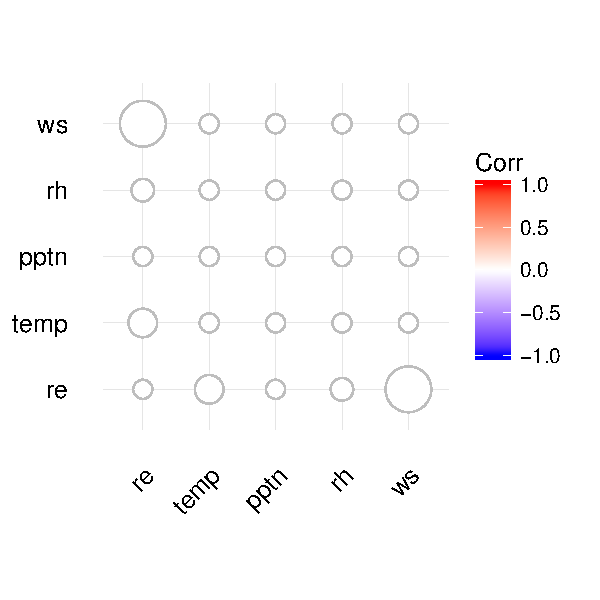
\includegraphics{../plots/cor_matrix}
    \vspace{-2em}
    \caption{Correlation matrix visualization.}
    \label{fig:cor_matrix}
\end{figure}
\vspace{-1em}
\begin{figure}[!ht]
    \center
    % !TEX encoding = UTF-8 Unicode
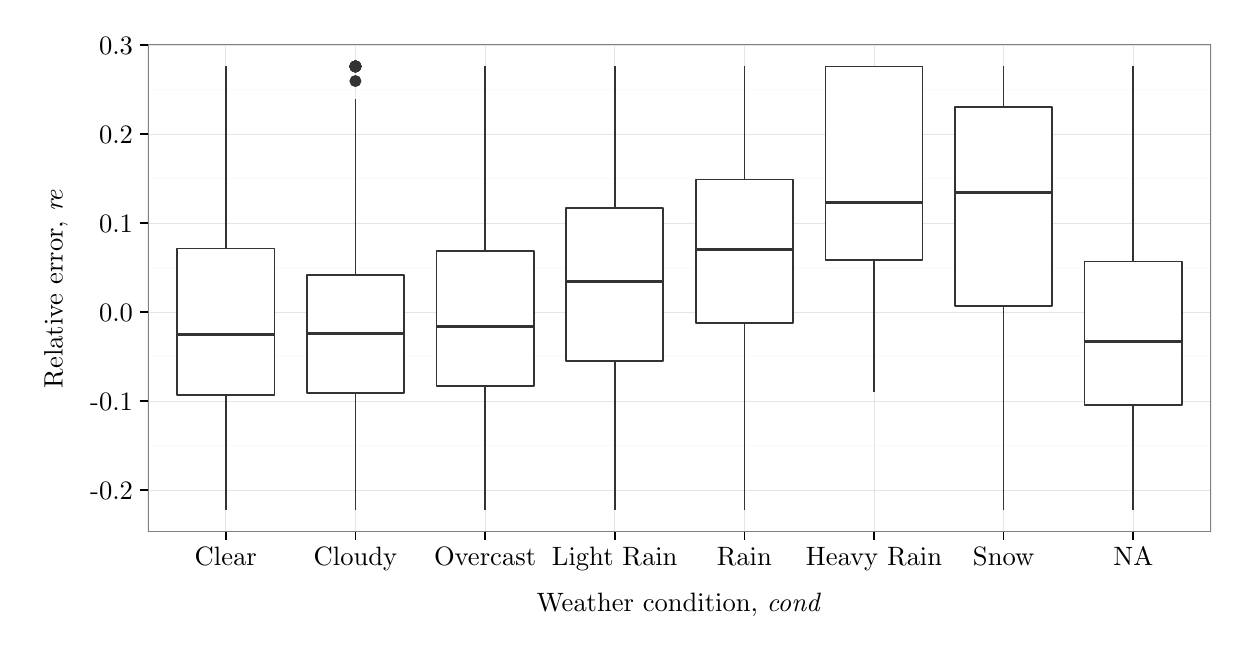
\begin{tikzpicture}[x=1pt,y=1pt]
\definecolor{fillColor}{RGB}{255,255,255}
\path[use as bounding box,fill=fillColor,fill opacity=0.00] (0,0) rectangle (433.62,216.81);
\begin{scope}
\path[clip] (  0.00,  0.00) rectangle (433.62,216.81);
\definecolor{drawColor}{RGB}{255,255,255}
\definecolor{fillColor}{RGB}{255,255,255}

\path[draw=drawColor,line width= 0.6pt,line join=round,line cap=round,fill=fillColor] (  0.00,  0.00) rectangle (433.62,216.81);
\end{scope}
\begin{scope}
\path[clip] ( 43.47, 34.62) rectangle (427.62,210.81);
\definecolor{fillColor}{RGB}{255,255,255}

\path[fill=fillColor] ( 43.47, 34.62) rectangle (427.62,210.81);
\definecolor{drawColor}{gray}{0.98}

\path[draw=drawColor,line width= 0.6pt,line join=round] ( 43.47, 65.84) --
	(427.62, 65.84);

\path[draw=drawColor,line width= 0.6pt,line join=round] ( 43.47, 98.00) --
	(427.62, 98.00);

\path[draw=drawColor,line width= 0.6pt,line join=round] ( 43.47,130.17) --
	(427.62,130.17);

\path[draw=drawColor,line width= 0.6pt,line join=round] ( 43.47,162.33) --
	(427.62,162.33);

\path[draw=drawColor,line width= 0.6pt,line join=round] ( 43.47,194.49) --
	(427.62,194.49);
\definecolor{drawColor}{gray}{0.90}

\path[draw=drawColor,line width= 0.2pt,line join=round] ( 43.47, 49.76) --
	(427.62, 49.76);

\path[draw=drawColor,line width= 0.2pt,line join=round] ( 43.47, 81.92) --
	(427.62, 81.92);

\path[draw=drawColor,line width= 0.2pt,line join=round] ( 43.47,114.08) --
	(427.62,114.08);

\path[draw=drawColor,line width= 0.2pt,line join=round] ( 43.47,146.25) --
	(427.62,146.25);

\path[draw=drawColor,line width= 0.2pt,line join=round] ( 43.47,178.41) --
	(427.62,178.41);

\path[draw=drawColor,line width= 0.2pt,line join=round] ( 43.47,210.57) --
	(427.62,210.57);

\path[draw=drawColor,line width= 0.2pt,line join=round] ( 71.58, 34.62) --
	( 71.58,210.81);

\path[draw=drawColor,line width= 0.2pt,line join=round] (118.43, 34.62) --
	(118.43,210.81);

\path[draw=drawColor,line width= 0.2pt,line join=round] (165.28, 34.62) --
	(165.28,210.81);

\path[draw=drawColor,line width= 0.2pt,line join=round] (212.12, 34.62) --
	(212.12,210.81);

\path[draw=drawColor,line width= 0.2pt,line join=round] (258.97, 34.62) --
	(258.97,210.81);

\path[draw=drawColor,line width= 0.2pt,line join=round] (305.82, 34.62) --
	(305.82,210.81);

\path[draw=drawColor,line width= 0.2pt,line join=round] (352.66, 34.62) --
	(352.66,210.81);

\path[draw=drawColor,line width= 0.2pt,line join=round] (399.51, 34.62) --
	(399.51,210.81);
\definecolor{drawColor}{gray}{0.20}

\path[draw=drawColor,line width= 0.6pt,line join=round] ( 71.58,136.97) -- ( 71.58,202.80);

\path[draw=drawColor,line width= 0.6pt,line join=round] ( 71.58, 84.19) -- ( 71.58, 42.63);

\path[draw=drawColor,line width= 0.6pt,line join=round,line cap=round,fill=fillColor] ( 54.02,136.97) --
	( 54.02, 84.19) --
	( 89.15, 84.19) --
	( 89.15,136.97) --
	( 54.02,136.97) --
	cycle;

\path[draw=drawColor,line width= 1.1pt,line join=round] ( 54.02,105.90) -- ( 89.15,105.90);
\definecolor{fillColor}{gray}{0.20}

\path[draw=drawColor,line width= 0.4pt,line join=round,line cap=round,fill=fillColor] (118.43,202.80) circle (  1.96);

\path[draw=drawColor,line width= 0.4pt,line join=round,line cap=round,fill=fillColor] (118.43,202.80) circle (  1.96);

\path[draw=drawColor,line width= 0.4pt,line join=round,line cap=round,fill=fillColor] (118.43,202.80) circle (  1.96);

\path[draw=drawColor,line width= 0.4pt,line join=round,line cap=round,fill=fillColor] (118.43,202.80) circle (  1.96);

\path[draw=drawColor,line width= 0.4pt,line join=round,line cap=round,fill=fillColor] (118.43,197.52) circle (  1.96);

\path[draw=drawColor,line width= 0.4pt,line join=round,line cap=round,fill=fillColor] (118.43,202.80) circle (  1.96);

\path[draw=drawColor,line width= 0.4pt,line join=round,line cap=round,fill=fillColor] (118.43,202.80) circle (  1.96);

\path[draw=drawColor,line width= 0.4pt,line join=round,line cap=round,fill=fillColor] (118.43,202.80) circle (  1.96);

\path[draw=drawColor,line width= 0.4pt,line join=round,line cap=round,fill=fillColor] (118.43,202.80) circle (  1.96);

\path[draw=drawColor,line width= 0.4pt,line join=round,line cap=round,fill=fillColor] (118.43,202.80) circle (  1.96);

\path[draw=drawColor,line width= 0.4pt,line join=round,line cap=round,fill=fillColor] (118.43,202.80) circle (  1.96);

\path[draw=drawColor,line width= 0.6pt,line join=round] (118.43,127.44) -- (118.43,191.09);

\path[draw=drawColor,line width= 0.6pt,line join=round] (118.43, 84.77) -- (118.43, 42.63);
\definecolor{fillColor}{RGB}{255,255,255}

\path[draw=drawColor,line width= 0.6pt,line join=round,line cap=round,fill=fillColor] (100.86,127.44) --
	(100.86, 84.77) --
	(136.00, 84.77) --
	(136.00,127.44) --
	(100.86,127.44) --
	cycle;

\path[draw=drawColor,line width= 1.1pt,line join=round] (100.86,106.45) -- (136.00,106.45);

\path[draw=drawColor,line width= 0.6pt,line join=round] (165.28,136.11) -- (165.28,202.80);

\path[draw=drawColor,line width= 0.6pt,line join=round] (165.28, 87.40) -- (165.28, 42.63);

\path[draw=drawColor,line width= 0.6pt,line join=round,line cap=round,fill=fillColor] (147.71,136.11) --
	(147.71, 87.40) --
	(182.84, 87.40) --
	(182.84,136.11) --
	(147.71,136.11) --
	cycle;

\path[draw=drawColor,line width= 1.1pt,line join=round] (147.71,108.82) -- (182.84,108.82);

\path[draw=drawColor,line width= 0.6pt,line join=round] (212.12,151.69) -- (212.12,202.80);

\path[draw=drawColor,line width= 0.6pt,line join=round] (212.12, 96.43) -- (212.12, 42.63);

\path[draw=drawColor,line width= 0.6pt,line join=round,line cap=round,fill=fillColor] (194.56,151.69) --
	(194.56, 96.43) --
	(229.69, 96.43) --
	(229.69,151.69) --
	(194.56,151.69) --
	cycle;

\path[draw=drawColor,line width= 1.1pt,line join=round] (194.56,125.17) -- (229.69,125.17);

\path[draw=drawColor,line width= 0.6pt,line join=round] (258.97,161.90) -- (258.97,202.80);

\path[draw=drawColor,line width= 0.6pt,line join=round] (258.97,110.03) -- (258.97, 42.63);

\path[draw=drawColor,line width= 0.6pt,line join=round,line cap=round,fill=fillColor] (241.40,161.90) --
	(241.40,110.03) --
	(276.54,110.03) --
	(276.54,161.90) --
	(241.40,161.90) --
	cycle;

\path[draw=drawColor,line width= 1.1pt,line join=round] (241.40,136.63) -- (276.54,136.63);

\path[draw=drawColor,line width= 0.6pt,line join=round] (305.82,202.80) -- (305.82,202.80);

\path[draw=drawColor,line width= 0.6pt,line join=round] (305.82,132.86) -- (305.82, 85.09);

\path[draw=drawColor,line width= 0.6pt,line join=round,line cap=round,fill=fillColor] (288.25,202.80) --
	(288.25,132.86) --
	(323.39,132.86) --
	(323.39,202.80) --
	(288.25,202.80) --
	cycle;

\path[draw=drawColor,line width= 1.1pt,line join=round] (288.25,153.56) -- (323.39,153.56);

\path[draw=drawColor,line width= 0.6pt,line join=round] (352.66,188.15) -- (352.66,202.80);

\path[draw=drawColor,line width= 0.6pt,line join=round] (352.66,116.22) -- (352.66, 42.63);

\path[draw=drawColor,line width= 0.6pt,line join=round,line cap=round,fill=fillColor] (335.10,188.15) --
	(335.10,116.22) --
	(370.23,116.22) --
	(370.23,188.15) --
	(335.10,188.15) --
	cycle;

\path[draw=drawColor,line width= 1.1pt,line join=round] (335.10,157.13) -- (370.23,157.13);

\path[draw=drawColor,line width= 0.6pt,line join=round] (399.51,132.34) -- (399.51,202.80);

\path[draw=drawColor,line width= 0.6pt,line join=round] (399.51, 80.57) -- (399.51, 42.63);

\path[draw=drawColor,line width= 0.6pt,line join=round,line cap=round,fill=fillColor] (381.94,132.34) --
	(381.94, 80.57) --
	(417.08, 80.57) --
	(417.08,132.34) --
	(381.94,132.34) --
	cycle;

\path[draw=drawColor,line width= 1.1pt,line join=round] (381.94,103.38) -- (417.08,103.38);
\definecolor{drawColor}{gray}{0.50}

\path[draw=drawColor,line width= 0.6pt,line join=round,line cap=round] ( 43.47, 34.62) rectangle (427.62,210.81);
\end{scope}
\begin{scope}
\path[clip] (  0.00,  0.00) rectangle (433.62,216.81);
\definecolor{drawColor}{RGB}{0,0,0}

\node[text=drawColor,anchor=base east,inner sep=0pt, outer sep=0pt, scale=  0.96] at ( 38.07, 46.45) {-0.2};

\node[text=drawColor,anchor=base east,inner sep=0pt, outer sep=0pt, scale=  0.96] at ( 38.07, 78.62) {-0.1};

\node[text=drawColor,anchor=base east,inner sep=0pt, outer sep=0pt, scale=  0.96] at ( 38.07,110.78) {0.0};

\node[text=drawColor,anchor=base east,inner sep=0pt, outer sep=0pt, scale=  0.96] at ( 38.07,142.94) {0.1};

\node[text=drawColor,anchor=base east,inner sep=0pt, outer sep=0pt, scale=  0.96] at ( 38.07,175.10) {0.2};

\node[text=drawColor,anchor=base east,inner sep=0pt, outer sep=0pt, scale=  0.96] at ( 38.07,207.27) {0.3};
\end{scope}
\begin{scope}
\path[clip] (  0.00,  0.00) rectangle (433.62,216.81);
\definecolor{drawColor}{RGB}{0,0,0}

\path[draw=drawColor,line width= 0.6pt,line join=round] ( 40.47, 49.76) --
	( 43.47, 49.76);

\path[draw=drawColor,line width= 0.6pt,line join=round] ( 40.47, 81.92) --
	( 43.47, 81.92);

\path[draw=drawColor,line width= 0.6pt,line join=round] ( 40.47,114.08) --
	( 43.47,114.08);

\path[draw=drawColor,line width= 0.6pt,line join=round] ( 40.47,146.25) --
	( 43.47,146.25);

\path[draw=drawColor,line width= 0.6pt,line join=round] ( 40.47,178.41) --
	( 43.47,178.41);

\path[draw=drawColor,line width= 0.6pt,line join=round] ( 40.47,210.57) --
	( 43.47,210.57);
\end{scope}
\begin{scope}
\path[clip] (  0.00,  0.00) rectangle (433.62,216.81);
\definecolor{drawColor}{RGB}{0,0,0}

\path[draw=drawColor,line width= 0.6pt,line join=round] ( 71.58, 31.62) --
	( 71.58, 34.62);

\path[draw=drawColor,line width= 0.6pt,line join=round] (118.43, 31.62) --
	(118.43, 34.62);

\path[draw=drawColor,line width= 0.6pt,line join=round] (165.28, 31.62) --
	(165.28, 34.62);

\path[draw=drawColor,line width= 0.6pt,line join=round] (212.12, 31.62) --
	(212.12, 34.62);

\path[draw=drawColor,line width= 0.6pt,line join=round] (258.97, 31.62) --
	(258.97, 34.62);

\path[draw=drawColor,line width= 0.6pt,line join=round] (305.82, 31.62) --
	(305.82, 34.62);

\path[draw=drawColor,line width= 0.6pt,line join=round] (352.66, 31.62) --
	(352.66, 34.62);

\path[draw=drawColor,line width= 0.6pt,line join=round] (399.51, 31.62) --
	(399.51, 34.62);
\end{scope}
\begin{scope}
\path[clip] (  0.00,  0.00) rectangle (433.62,216.81);
\definecolor{drawColor}{RGB}{0,0,0}

\node[text=drawColor,anchor=base,inner sep=0pt, outer sep=0pt, scale=  0.96] at ( 71.58, 22.61) {Clear};

\node[text=drawColor,anchor=base,inner sep=0pt, outer sep=0pt, scale=  0.96] at (118.43, 22.61) {Cloudy};

\node[text=drawColor,anchor=base,inner sep=0pt, outer sep=0pt, scale=  0.96] at (165.28, 22.61) {Overcast};

\node[text=drawColor,anchor=base,inner sep=0pt, outer sep=0pt, scale=  0.96] at (212.12, 22.61) {Light Rain};

\node[text=drawColor,anchor=base,inner sep=0pt, outer sep=0pt, scale=  0.96] at (258.97, 22.61) {Rain};

\node[text=drawColor,anchor=base,inner sep=0pt, outer sep=0pt, scale=  0.96] at (305.82, 22.61) {Heavy Rain};

\node[text=drawColor,anchor=base,inner sep=0pt, outer sep=0pt, scale=  0.96] at (352.66, 22.61) {Snow};

\node[text=drawColor,anchor=base,inner sep=0pt, outer sep=0pt, scale=  0.96] at (399.51, 22.61) {NA};
\end{scope}
\begin{scope}
\path[clip] (  0.00,  0.00) rectangle (433.62,216.81);
\definecolor{drawColor}{RGB}{0,0,0}

\node[text=drawColor,anchor=base,inner sep=0pt, outer sep=0pt, scale=  0.96] at (235.55,  6.00) {Weather condition, $\mathit{cond}$};
\end{scope}
\begin{scope}
\path[clip] (  0.00,  0.00) rectangle (433.62,216.81);
\definecolor{drawColor}{RGB}{0,0,0}

\node[text=drawColor,rotate= 90.00,anchor=base,inner sep=0pt, outer sep=0pt, scale=  0.96] at ( 12.61,122.72) {Relative error, $\mathit{re}$};
\end{scope}
\end{tikzpicture}

    \vspace{-1em}
    \caption{Correlation between weather conditions and relative error.}
    \label{fig:cor_cond}
\end{figure}
\vspace{-1em}

\begin{figure}[!ht]
    \center
    % !TEX encoding = UTF-8 Unicode
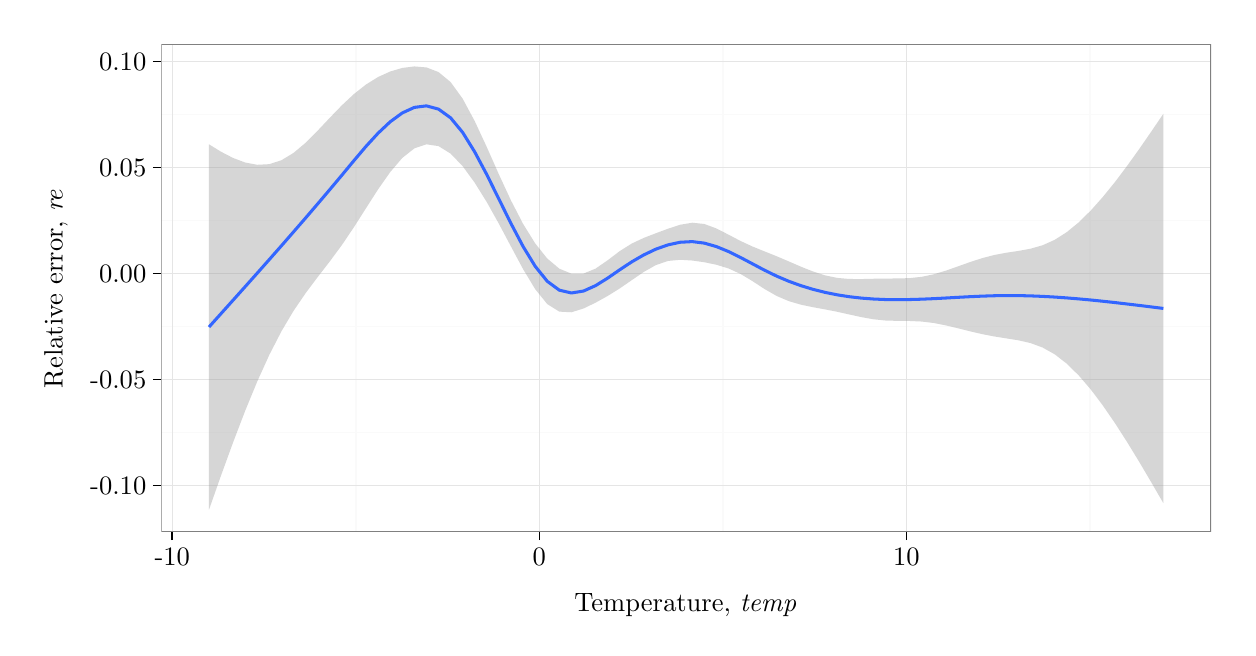
\begin{tikzpicture}[x=1pt,y=1pt]
\definecolor{fillColor}{RGB}{255,255,255}
\path[use as bounding box,fill=fillColor,fill opacity=0.00] (0,0) rectangle (433.62,216.81);
\begin{scope}
\path[clip] (  0.00,  0.00) rectangle (433.62,216.81);
\definecolor{drawColor}{RGB}{255,255,255}
\definecolor{fillColor}{RGB}{255,255,255}

\path[draw=drawColor,line width= 0.6pt,line join=round,line cap=round,fill=fillColor] (  0.00,  0.00) rectangle (433.62,216.81);
\end{scope}
\begin{scope}
\path[clip] ( 48.27, 34.62) rectangle (427.62,210.81);
\definecolor{fillColor}{RGB}{255,255,255}

\path[fill=fillColor] ( 48.27, 34.62) rectangle (427.62,210.81);
\definecolor{drawColor}{gray}{0.98}

\path[draw=drawColor,line width= 0.6pt,line join=round] ( 48.27, 70.57) --
	(427.62, 70.57);

\path[draw=drawColor,line width= 0.6pt,line join=round] ( 48.27,108.88) --
	(427.62,108.88);

\path[draw=drawColor,line width= 0.6pt,line join=round] ( 48.27,147.18) --
	(427.62,147.18);

\path[draw=drawColor,line width= 0.6pt,line join=round] ( 48.27,185.49) --
	(427.62,185.49);

\path[draw=drawColor,line width= 0.6pt,line join=round] (118.57, 34.62) --
	(118.57,210.81);

\path[draw=drawColor,line width= 0.6pt,line join=round] (251.21, 34.62) --
	(251.21,210.81);

\path[draw=drawColor,line width= 0.6pt,line join=round] (383.85, 34.62) --
	(383.85,210.81);
\definecolor{drawColor}{gray}{0.90}

\path[draw=drawColor,line width= 0.2pt,line join=round] ( 48.27, 51.42) --
	(427.62, 51.42);

\path[draw=drawColor,line width= 0.2pt,line join=round] ( 48.27, 89.73) --
	(427.62, 89.73);

\path[draw=drawColor,line width= 0.2pt,line join=round] ( 48.27,128.03) --
	(427.62,128.03);

\path[draw=drawColor,line width= 0.2pt,line join=round] ( 48.27,166.34) --
	(427.62,166.34);

\path[draw=drawColor,line width= 0.2pt,line join=round] ( 48.27,204.64) --
	(427.62,204.64);

\path[draw=drawColor,line width= 0.2pt,line join=round] ( 52.25, 34.62) --
	( 52.25,210.81);

\path[draw=drawColor,line width= 0.2pt,line join=round] (184.89, 34.62) --
	(184.89,210.81);

\path[draw=drawColor,line width= 0.2pt,line join=round] (317.53, 34.62) --
	(317.53,210.81);
\definecolor{fillColor}{RGB}{153,153,153}

\path[fill=fillColor,fill opacity=0.40] ( 65.52,174.65) --
	( 69.88,171.97) --
	( 74.25,169.71) --
	( 78.61,168.07) --
	( 82.98,167.26) --
	( 87.34,167.49) --
	( 91.71,168.91) --
	( 96.07,171.55) --
	(100.44,175.22) --
	(104.80,179.60) --
	(109.17,184.24) --
	(113.54,188.76) --
	(117.90,192.83) --
	(122.27,196.27) --
	(126.63,198.98) --
	(131.00,200.97) --
	(135.36,202.25) --
	(139.73,202.80) --
	(144.09,202.44) --
	(148.46,200.76) --
	(152.82,197.16) --
	(157.19,191.12) --
	(161.55,183.01) --
	(165.92,173.61) --
	(170.28,163.77) --
	(174.65,154.33) --
	(179.01,145.91) --
	(183.38,138.86) --
	(187.75,133.39) --
	(192.11,129.72) --
	(196.48,127.92) --
	(200.84,127.95) --
	(205.21,129.74) --
	(209.57,132.75) --
	(213.94,136.07) --
	(218.30,138.81) --
	(222.67,140.85) --
	(227.03,142.54) --
	(231.40,144.16) --
	(235.76,145.59) --
	(240.13,146.33) --
	(244.49,145.87) --
	(248.86,144.26) --
	(253.23,142.02) --
	(257.59,139.73) --
	(261.96,137.71) --
	(266.32,135.94) --
	(270.69,134.19) --
	(275.05,132.33) --
	(279.42,130.44) --
	(283.78,128.70) --
	(288.15,127.30) --
	(292.51,126.39) --
	(296.88,126.00) --
	(301.24,125.97) --
	(305.61,126.08) --
	(309.97,126.16) --
	(314.34,126.18) --
	(318.71,126.31) --
	(323.07,126.78) --
	(327.44,127.70) --
	(331.80,129.01) --
	(336.17,130.55) --
	(340.53,132.11) --
	(344.90,133.52) --
	(349.26,134.66) --
	(353.63,135.48) --
	(357.99,136.13) --
	(362.36,136.93) --
	(366.72,138.17) --
	(371.09,140.13) --
	(375.45,142.90) --
	(379.82,146.48) --
	(384.19,150.78) --
	(388.55,155.68) --
	(392.92,161.07) --
	(397.28,166.86) --
	(401.65,172.95) --
	(406.01,179.26) --
	(410.38,185.70) --
	(410.38, 44.99) --
	(406.01, 52.53) --
	(401.65, 59.92) --
	(397.28, 67.07) --
	(392.92, 73.87) --
	(388.55, 80.22) --
	(384.19, 86.02) --
	(379.82, 91.12) --
	(375.45, 95.42) --
	(371.09, 98.80) --
	(366.72,101.24) --
	(362.36,102.85) --
	(357.99,103.84) --
	(353.63,104.54) --
	(349.26,105.23) --
	(344.90,106.08) --
	(340.53,107.09) --
	(336.17,108.18) --
	(331.80,109.23) --
	(327.44,110.09) --
	(323.07,110.62) --
	(318.71,110.82) --
	(314.34,110.86) --
	(309.97,110.99) --
	(305.61,111.44) --
	(301.24,112.22) --
	(296.88,113.18) --
	(292.51,114.15) --
	(288.15,115.01) --
	(283.78,115.80) --
	(279.42,116.71) --
	(275.05,117.99) --
	(270.69,119.84) --
	(266.32,122.34) --
	(261.96,125.19) --
	(257.59,127.82) --
	(253.23,129.81) --
	(248.86,131.15) --
	(244.49,132.05) --
	(240.13,132.67) --
	(235.76,132.94) --
	(231.40,132.51) --
	(227.03,131.04) --
	(222.67,128.58) --
	(218.30,125.59) --
	(213.94,122.58) --
	(209.57,119.86) --
	(205.21,117.44) --
	(200.84,115.33) --
	(196.48,113.97) --
	(192.11,114.20) --
	(187.75,116.93) --
	(183.38,122.34) --
	(179.01,129.58) --
	(174.65,137.72) --
	(170.28,145.95) --
	(165.92,153.74) --
	(161.55,160.77) --
	(157.19,166.76) --
	(152.82,171.31) --
	(148.46,174.01) --
	(144.09,174.66) --
	(139.73,173.19) --
	(135.36,169.73) --
	(131.00,164.63) --
	(126.63,158.40) --
	(122.27,151.60) --
	(117.90,144.74) --
	(113.54,138.27) --
	(109.17,132.35) --
	(104.80,126.70) --
	(100.44,120.89) --
	( 96.07,114.48) --
	( 91.71,107.13) --
	( 87.34, 98.64) --
	( 82.98, 89.02) --
	( 78.61, 78.42) --
	( 74.25, 67.02) --
	( 69.88, 55.03) --
	( 65.52, 42.63) --
	cycle;
\definecolor{drawColor}{RGB}{51,102,255}

\path[draw=drawColor,line width= 1.1pt,line join=round] ( 65.52,108.64) --
	( 69.88,113.50) --
	( 74.25,118.37) --
	( 78.61,123.24) --
	( 82.98,128.14) --
	( 87.34,133.06) --
	( 91.71,138.02) --
	( 96.07,143.02) --
	(100.44,148.06) --
	(104.80,153.15) --
	(109.17,158.30) --
	(113.54,163.51) --
	(117.90,168.78) --
	(122.27,173.93) --
	(126.63,178.69) --
	(131.00,182.80) --
	(135.36,185.99) --
	(139.73,188.00) --
	(144.09,188.55) --
	(148.46,187.38) --
	(152.82,184.23) --
	(157.19,178.94) --
	(161.55,171.89) --
	(165.92,163.68) --
	(170.28,154.86) --
	(174.65,146.03) --
	(179.01,137.75) --
	(183.38,130.60) --
	(187.75,125.16) --
	(192.11,121.96) --
	(196.48,120.94) --
	(200.84,121.64) --
	(205.21,123.59) --
	(209.57,126.31) --
	(213.94,129.32) --
	(218.30,132.20) --
	(222.67,134.72) --
	(227.03,136.79) --
	(231.40,138.33) --
	(235.76,139.27) --
	(240.13,139.50) --
	(244.49,138.96) --
	(248.86,137.71) --
	(253.23,135.92) --
	(257.59,133.77) --
	(261.96,131.45) --
	(266.32,129.14) --
	(270.69,127.01) --
	(275.05,125.16) --
	(279.42,123.58) --
	(283.78,122.25) --
	(288.15,121.15) --
	(292.51,120.27) --
	(296.88,119.59) --
	(301.24,119.09) --
	(305.61,118.76) --
	(309.97,118.57) --
	(314.34,118.52) --
	(318.71,118.57) --
	(323.07,118.70) --
	(327.44,118.89) --
	(331.80,119.12) --
	(336.17,119.37) --
	(340.53,119.60) --
	(344.90,119.80) --
	(349.26,119.94) --
	(353.63,120.01) --
	(357.99,119.99) --
	(362.36,119.89) --
	(366.72,119.71) --
	(371.09,119.47) --
	(375.45,119.16) --
	(379.82,118.80) --
	(384.19,118.40) --
	(388.55,117.95) --
	(392.92,117.47) --
	(397.28,116.96) --
	(401.65,116.44) --
	(406.01,115.90) --
	(410.38,115.35);
\definecolor{drawColor}{gray}{0.50}

\path[draw=drawColor,line width= 0.6pt,line join=round,line cap=round] ( 48.27, 34.62) rectangle (427.62,210.81);
\end{scope}
\begin{scope}
\path[clip] (  0.00,  0.00) rectangle (433.62,216.81);
\definecolor{drawColor}{RGB}{0,0,0}

\node[text=drawColor,anchor=base east,inner sep=0pt, outer sep=0pt, scale=  0.96] at ( 42.87, 48.11) {-0.10};

\node[text=drawColor,anchor=base east,inner sep=0pt, outer sep=0pt, scale=  0.96] at ( 42.87, 86.42) {-0.05};

\node[text=drawColor,anchor=base east,inner sep=0pt, outer sep=0pt, scale=  0.96] at ( 42.87,124.72) {0.00};

\node[text=drawColor,anchor=base east,inner sep=0pt, outer sep=0pt, scale=  0.96] at ( 42.87,163.03) {0.05};

\node[text=drawColor,anchor=base east,inner sep=0pt, outer sep=0pt, scale=  0.96] at ( 42.87,201.33) {0.10};
\end{scope}
\begin{scope}
\path[clip] (  0.00,  0.00) rectangle (433.62,216.81);
\definecolor{drawColor}{RGB}{0,0,0}

\path[draw=drawColor,line width= 0.6pt,line join=round] ( 45.27, 51.42) --
	( 48.27, 51.42);

\path[draw=drawColor,line width= 0.6pt,line join=round] ( 45.27, 89.73) --
	( 48.27, 89.73);

\path[draw=drawColor,line width= 0.6pt,line join=round] ( 45.27,128.03) --
	( 48.27,128.03);

\path[draw=drawColor,line width= 0.6pt,line join=round] ( 45.27,166.34) --
	( 48.27,166.34);

\path[draw=drawColor,line width= 0.6pt,line join=round] ( 45.27,204.64) --
	( 48.27,204.64);
\end{scope}
\begin{scope}
\path[clip] (  0.00,  0.00) rectangle (433.62,216.81);
\definecolor{drawColor}{RGB}{0,0,0}

\path[draw=drawColor,line width= 0.6pt,line join=round] ( 52.25, 31.62) --
	( 52.25, 34.62);

\path[draw=drawColor,line width= 0.6pt,line join=round] (184.89, 31.62) --
	(184.89, 34.62);

\path[draw=drawColor,line width= 0.6pt,line join=round] (317.53, 31.62) --
	(317.53, 34.62);
\end{scope}
\begin{scope}
\path[clip] (  0.00,  0.00) rectangle (433.62,216.81);
\definecolor{drawColor}{RGB}{0,0,0}

\node[text=drawColor,anchor=base,inner sep=0pt, outer sep=0pt, scale=  0.96] at ( 52.25, 22.61) {-10};

\node[text=drawColor,anchor=base,inner sep=0pt, outer sep=0pt, scale=  0.96] at (184.89, 22.61) {0};

\node[text=drawColor,anchor=base,inner sep=0pt, outer sep=0pt, scale=  0.96] at (317.53, 22.61) {10};
\end{scope}
\begin{scope}
\path[clip] (  0.00,  0.00) rectangle (433.62,216.81);
\definecolor{drawColor}{RGB}{0,0,0}

\node[text=drawColor,anchor=base,inner sep=0pt, outer sep=0pt, scale=  0.96] at (237.95,  6.00) {Temperature, $\mathit{temp}$};
\end{scope}
\begin{scope}
\path[clip] (  0.00,  0.00) rectangle (433.62,216.81);
\definecolor{drawColor}{RGB}{0,0,0}

\node[text=drawColor,rotate= 90.00,anchor=base,inner sep=0pt, outer sep=0pt, scale=  0.96] at ( 12.61,122.72) {Relative error, $\mathit{re}$};
\end{scope}
\end{tikzpicture}

    \vspace{-1em}
    \caption{Correlation between temperature and relative error.}
    \label{fig:cor_temp}
\end{figure}

\begin{figure}[!ht]
    \center
    % !TEX encoding = UTF-8 Unicode
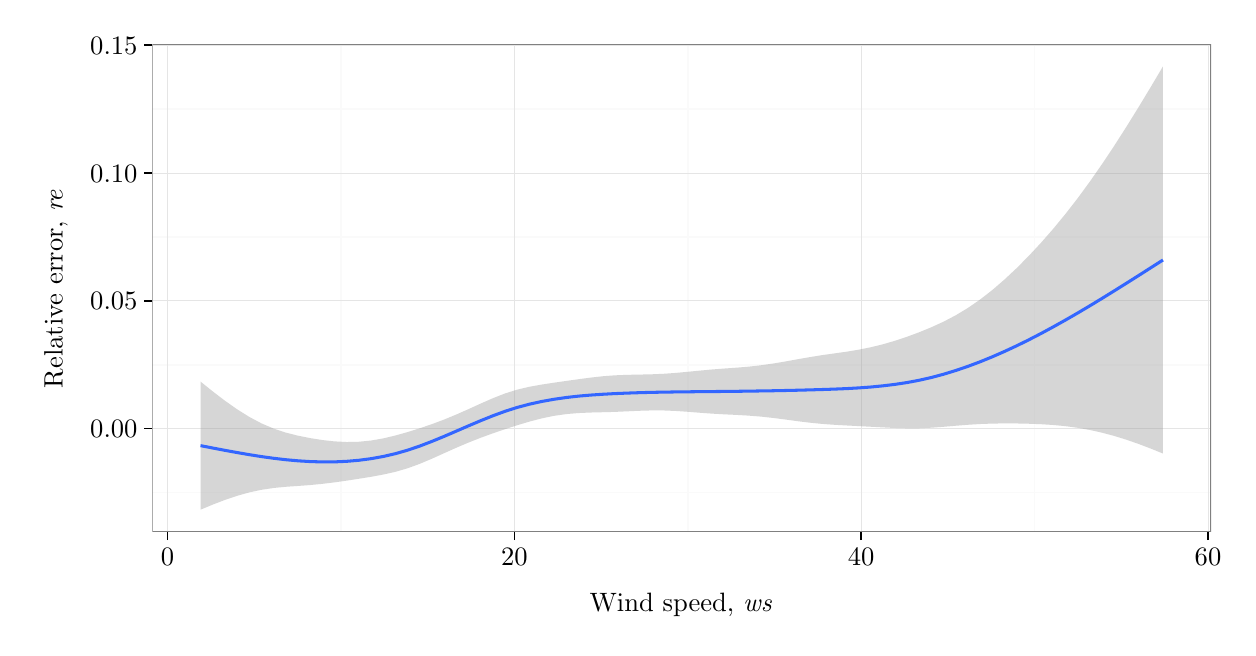
\begin{tikzpicture}[x=1pt,y=1pt]
\definecolor{fillColor}{RGB}{255,255,255}
\path[use as bounding box,fill=fillColor,fill opacity=0.00] (0,0) rectangle (433.62,216.81);
\begin{scope}
\path[clip] (  0.00,  0.00) rectangle (433.62,216.81);
\definecolor{drawColor}{RGB}{255,255,255}
\definecolor{fillColor}{RGB}{255,255,255}

\path[draw=drawColor,line width= 0.6pt,line join=round,line cap=round,fill=fillColor] (  0.00,  0.00) rectangle (433.62,216.81);
\end{scope}
\begin{scope}
\path[clip] ( 45.07, 34.62) rectangle (427.62,210.81);
\definecolor{fillColor}{RGB}{255,255,255}

\path[fill=fillColor] ( 45.07, 34.62) rectangle (427.62,210.81);
\definecolor{drawColor}{gray}{0.98}

\path[draw=drawColor,line width= 0.6pt,line join=round] ( 45.07, 48.83) --
	(427.62, 48.83);

\path[draw=drawColor,line width= 0.6pt,line join=round] ( 45.07, 95.03) --
	(427.62, 95.03);

\path[draw=drawColor,line width= 0.6pt,line join=round] ( 45.07,141.23) --
	(427.62,141.23);

\path[draw=drawColor,line width= 0.6pt,line join=round] ( 45.07,187.44) --
	(427.62,187.44);

\path[draw=drawColor,line width= 0.6pt,line join=round] (113.22, 34.62) --
	(113.22,210.81);

\path[draw=drawColor,line width= 0.6pt,line join=round] (238.54, 34.62) --
	(238.54,210.81);

\path[draw=drawColor,line width= 0.6pt,line join=round] (363.86, 34.62) --
	(363.86,210.81);
\definecolor{drawColor}{gray}{0.90}

\path[draw=drawColor,line width= 0.2pt,line join=round] ( 45.07, 71.93) --
	(427.62, 71.93);

\path[draw=drawColor,line width= 0.2pt,line join=round] ( 45.07,118.13) --
	(427.62,118.13);

\path[draw=drawColor,line width= 0.2pt,line join=round] ( 45.07,164.34) --
	(427.62,164.34);

\path[draw=drawColor,line width= 0.2pt,line join=round] ( 45.07,210.54) --
	(427.62,210.54);

\path[draw=drawColor,line width= 0.2pt,line join=round] ( 50.56, 34.62) --
	( 50.56,210.81);

\path[draw=drawColor,line width= 0.2pt,line join=round] (175.88, 34.62) --
	(175.88,210.81);

\path[draw=drawColor,line width= 0.2pt,line join=round] (301.20, 34.62) --
	(301.20,210.81);

\path[draw=drawColor,line width= 0.2pt,line join=round] (426.52, 34.62) --
	(426.52,210.81);
\definecolor{fillColor}{RGB}{153,153,153}

\path[fill=fillColor,fill opacity=0.40] ( 62.46, 88.93) --
	( 66.86, 85.38) --
	( 71.27, 82.01) --
	( 75.67, 78.91) --
	( 80.07, 76.16) --
	( 84.47, 73.82) --
	( 88.88, 71.94) --
	( 93.28, 70.48) --
	( 97.68, 69.37) --
	(102.08, 68.49) --
	(106.48, 67.80) --
	(110.89, 67.31) --
	(115.29, 67.08) --
	(119.69, 67.18) --
	(124.09, 67.62) --
	(128.49, 68.39) --
	(132.90, 69.44) --
	(137.30, 70.68) --
	(141.70, 72.05) --
	(146.10, 73.56) --
	(150.51, 75.21) --
	(154.91, 77.03) --
	(159.31, 78.97) --
	(163.71, 80.98) --
	(168.11, 82.91) --
	(172.52, 84.64) --
	(176.92, 86.02) --
	(181.32, 87.05) --
	(185.72, 87.84) --
	(190.12, 88.51) --
	(194.53, 89.14) --
	(198.93, 89.76) --
	(203.33, 90.35) --
	(207.73, 90.84) --
	(212.14, 91.18) --
	(216.54, 91.36) --
	(220.94, 91.45) --
	(225.34, 91.55) --
	(229.74, 91.74) --
	(234.15, 92.05) --
	(238.55, 92.46) --
	(242.95, 92.89) --
	(247.35, 93.30) --
	(251.75, 93.64) --
	(256.16, 93.95) --
	(260.56, 94.32) --
	(264.96, 94.81) --
	(269.36, 95.44) --
	(273.77, 96.18) --
	(278.17, 96.98) --
	(282.57, 97.75) --
	(286.97, 98.46) --
	(291.37, 99.08) --
	(295.78, 99.70) --
	(300.18,100.42) --
	(304.58,101.30) --
	(308.98,102.38) --
	(313.38,103.66) --
	(317.79,105.13) --
	(322.19,106.76) --
	(326.59,108.57) --
	(330.99,110.59) --
	(335.40,112.90) --
	(339.80,115.56) --
	(344.20,118.60) --
	(348.60,122.03) --
	(353.00,125.83) --
	(357.41,129.96) --
	(361.81,134.40) --
	(366.21,139.13) --
	(370.61,144.16) --
	(375.01,149.51) --
	(379.42,155.18) --
	(383.82,161.19) --
	(388.22,167.51) --
	(392.62,174.12) --
	(397.03,181.00) --
	(401.43,188.10) --
	(405.83,195.38) --
	(410.23,202.80) --
	(410.23, 62.93) --
	(405.83, 64.71) --
	(401.43, 66.39) --
	(397.03, 67.92) --
	(392.62, 69.28) --
	(388.22, 70.46) --
	(383.82, 71.44) --
	(379.42, 72.22) --
	(375.01, 72.82) --
	(370.61, 73.24) --
	(366.21, 73.52) --
	(361.81, 73.69) --
	(357.41, 73.79) --
	(353.00, 73.81) --
	(348.60, 73.75) --
	(344.20, 73.59) --
	(339.80, 73.32) --
	(335.40, 72.97) --
	(330.99, 72.59) --
	(326.59, 72.26) --
	(322.19, 72.06) --
	(317.79, 72.04) --
	(313.38, 72.16) --
	(308.98, 72.37) --
	(304.58, 72.61) --
	(300.18, 72.84) --
	(295.78, 73.07) --
	(291.37, 73.32) --
	(286.97, 73.64) --
	(282.57, 74.08) --
	(278.17, 74.62) --
	(273.77, 75.22) --
	(269.36, 75.79) --
	(264.96, 76.27) --
	(260.56, 76.62) --
	(256.16, 76.88) --
	(251.75, 77.09) --
	(247.35, 77.34) --
	(242.95, 77.66) --
	(238.55, 78.01) --
	(234.15, 78.31) --
	(229.74, 78.49) --
	(225.34, 78.50) --
	(220.94, 78.37) --
	(216.54, 78.17) --
	(212.14, 77.97) --
	(207.73, 77.85) --
	(203.33, 77.74) --
	(198.93, 77.55) --
	(194.53, 77.17) --
	(190.12, 76.54) --
	(185.72, 75.62) --
	(181.32, 74.47) --
	(176.92, 73.16) --
	(172.52, 71.74) --
	(168.11, 70.23) --
	(163.71, 68.63) --
	(159.31, 66.90) --
	(154.91, 65.03) --
	(150.51, 63.06) --
	(146.10, 61.07) --
	(141.70, 59.21) --
	(137.30, 57.60) --
	(132.90, 56.32) --
	(128.49, 55.33) --
	(124.09, 54.52) --
	(119.69, 53.81) --
	(115.29, 53.13) --
	(110.89, 52.51) --
	(106.48, 51.97) --
	(102.08, 51.54) --
	( 97.68, 51.21) --
	( 93.28, 50.91) --
	( 88.88, 50.48) --
	( 84.47, 49.82) --
	( 80.07, 48.88) --
	( 75.67, 47.65) --
	( 71.27, 46.16) --
	( 66.86, 44.47) --
	( 62.46, 42.63) --
	cycle;
\definecolor{drawColor}{RGB}{51,102,255}

\path[draw=drawColor,line width= 1.1pt,line join=round] ( 62.46, 65.78) --
	( 66.86, 64.92) --
	( 71.27, 64.08) --
	( 75.67, 63.28) --
	( 80.07, 62.52) --
	( 84.47, 61.82) --
	( 88.88, 61.21) --
	( 93.28, 60.69) --
	( 97.68, 60.29) --
	(102.08, 60.02) --
	(106.48, 59.89) --
	(110.89, 59.91) --
	(115.29, 60.11) --
	(119.69, 60.49) --
	(124.09, 61.07) --
	(128.49, 61.86) --
	(132.90, 62.88) --
	(137.30, 64.14) --
	(141.70, 65.63) --
	(146.10, 67.32) --
	(150.51, 69.13) --
	(154.91, 71.03) --
	(159.31, 72.94) --
	(163.71, 74.80) --
	(168.11, 76.57) --
	(172.52, 78.19) --
	(176.92, 79.59) --
	(181.32, 80.76) --
	(185.72, 81.73) --
	(190.12, 82.52) --
	(194.53, 83.16) --
	(198.93, 83.66) --
	(203.33, 84.04) --
	(207.73, 84.34) --
	(212.14, 84.58) --
	(216.54, 84.76) --
	(220.94, 84.91) --
	(225.34, 85.03) --
	(229.74, 85.11) --
	(234.15, 85.18) --
	(238.55, 85.23) --
	(242.95, 85.28) --
	(247.35, 85.32) --
	(251.75, 85.36) --
	(256.16, 85.41) --
	(260.56, 85.47) --
	(264.96, 85.54) --
	(269.36, 85.61) --
	(273.77, 85.70) --
	(278.17, 85.80) --
	(282.57, 85.92) --
	(286.97, 86.05) --
	(291.37, 86.20) --
	(295.78, 86.38) --
	(300.18, 86.63) --
	(304.58, 86.95) --
	(308.98, 87.38) --
	(313.38, 87.91) --
	(317.79, 88.58) --
	(322.19, 89.41) --
	(326.59, 90.41) --
	(330.99, 91.59) --
	(335.40, 92.94) --
	(339.80, 94.44) --
	(344.20, 96.09) --
	(348.60, 97.89) --
	(353.00, 99.82) --
	(357.41,101.87) --
	(361.81,104.04) --
	(366.21,106.32) --
	(370.61,108.70) --
	(375.01,111.16) --
	(379.42,113.70) --
	(383.82,116.31) --
	(388.22,118.98) --
	(392.62,121.70) --
	(397.03,124.46) --
	(401.43,127.24) --
	(405.83,130.05) --
	(410.23,132.86);
\definecolor{drawColor}{gray}{0.50}

\path[draw=drawColor,line width= 0.6pt,line join=round,line cap=round] ( 45.07, 34.62) rectangle (427.62,210.81);
\end{scope}
\begin{scope}
\path[clip] (  0.00,  0.00) rectangle (433.62,216.81);
\definecolor{drawColor}{RGB}{0,0,0}

\node[text=drawColor,anchor=base east,inner sep=0pt, outer sep=0pt, scale=  0.96] at ( 39.67, 68.63) {0.00};

\node[text=drawColor,anchor=base east,inner sep=0pt, outer sep=0pt, scale=  0.96] at ( 39.67,114.83) {0.05};

\node[text=drawColor,anchor=base east,inner sep=0pt, outer sep=0pt, scale=  0.96] at ( 39.67,161.03) {0.10};

\node[text=drawColor,anchor=base east,inner sep=0pt, outer sep=0pt, scale=  0.96] at ( 39.67,207.23) {0.15};
\end{scope}
\begin{scope}
\path[clip] (  0.00,  0.00) rectangle (433.62,216.81);
\definecolor{drawColor}{RGB}{0,0,0}

\path[draw=drawColor,line width= 0.6pt,line join=round] ( 42.07, 71.93) --
	( 45.07, 71.93);

\path[draw=drawColor,line width= 0.6pt,line join=round] ( 42.07,118.13) --
	( 45.07,118.13);

\path[draw=drawColor,line width= 0.6pt,line join=round] ( 42.07,164.34) --
	( 45.07,164.34);

\path[draw=drawColor,line width= 0.6pt,line join=round] ( 42.07,210.54) --
	( 45.07,210.54);
\end{scope}
\begin{scope}
\path[clip] (  0.00,  0.00) rectangle (433.62,216.81);
\definecolor{drawColor}{RGB}{0,0,0}

\path[draw=drawColor,line width= 0.6pt,line join=round] ( 50.56, 31.62) --
	( 50.56, 34.62);

\path[draw=drawColor,line width= 0.6pt,line join=round] (175.88, 31.62) --
	(175.88, 34.62);

\path[draw=drawColor,line width= 0.6pt,line join=round] (301.20, 31.62) --
	(301.20, 34.62);

\path[draw=drawColor,line width= 0.6pt,line join=round] (426.52, 31.62) --
	(426.52, 34.62);
\end{scope}
\begin{scope}
\path[clip] (  0.00,  0.00) rectangle (433.62,216.81);
\definecolor{drawColor}{RGB}{0,0,0}

\node[text=drawColor,anchor=base,inner sep=0pt, outer sep=0pt, scale=  0.96] at ( 50.56, 22.61) {0};

\node[text=drawColor,anchor=base,inner sep=0pt, outer sep=0pt, scale=  0.96] at (175.88, 22.61) {20};

\node[text=drawColor,anchor=base,inner sep=0pt, outer sep=0pt, scale=  0.96] at (301.20, 22.61) {40};

\node[text=drawColor,anchor=base,inner sep=0pt, outer sep=0pt, scale=  0.96] at (426.52, 22.61) {60};
\end{scope}
\begin{scope}
\path[clip] (  0.00,  0.00) rectangle (433.62,216.81);
\definecolor{drawColor}{RGB}{0,0,0}

\node[text=drawColor,anchor=base,inner sep=0pt, outer sep=0pt, scale=  0.96] at (236.35,  6.00) {Wind speed, $\mathit{ws}$};
\end{scope}
\begin{scope}
\path[clip] (  0.00,  0.00) rectangle (433.62,216.81);
\definecolor{drawColor}{RGB}{0,0,0}

\node[text=drawColor,rotate= 90.00,anchor=base,inner sep=0pt, outer sep=0pt, scale=  0.96] at ( 12.61,122.72) {Relative error, $\mathit{re}$};
\end{scope}
\end{tikzpicture}

    \caption{Correlation between wind speed and relative error.}
    \label{fig:cor_ws}
\end{figure}

\subsection{Principal component analysis}
As  \emph{Principal component analysis} (PCA) only works on continues variables a series of dummy-variables is introduced for the discrete variable weather condition \gls{cond_i}, while day type, \gls{daytype_i}, and peek class, \gls{peek_i} is dropped since their contribution is non-significant cf. previous section. The PCA is only done on the weather data, and loadings is then colored by travel demand deviation, \gls{re_i}.

The dummy transformation yields a data set of total of 11 variables, which is mean centered and scaled before PCA is applied. The scree plot of the resulting 11 principal components (PC) is shown \Cref{fig:pca_screeplot}. Already from the scree plot it is evident, that the total explained variance increases quite slowly as principal components are included. Thus it suggest that the weather data set is not modeled well by the hyper-projection onto the reduced space of the PCA.

Nevertheless the loadings plots is colored cf.\ \gls{re_i} and inspected. Since comparing all 11 principal components would yield 55 loadings plots, only the first 5 principal components are selected, resulting in the 10 loadings plots shown in \Cref{fig:pca_loadings}, where a blue color corresponds to a positive value of \gls{re_i} (increased demand), and red to a negative value of \gls{re_i} (decreased demand).

It is hard to argue about any clear patterns in the loadings plots. The clusters formed are in all cases due to the dummy variables. Even though clusters of different kind of rains, e.g.\ as seen in PC3/PC5-plot, are more blue then the cloudy and overcast clusters, it really does not capture the multivariate correlation better than the boxplot in~\Cref{fig:cor_cond}. PCA has also been tried without the dummy-variables, but it yields only cloudy loadings plot with just as little separation between increased and decreased demand.

For this reason it is argued that PCA is not an appropriate method for the multivariate analysis.
\begin{figure}[!ht]
    \center
    % !TEX encoding = UTF-8 Unicode
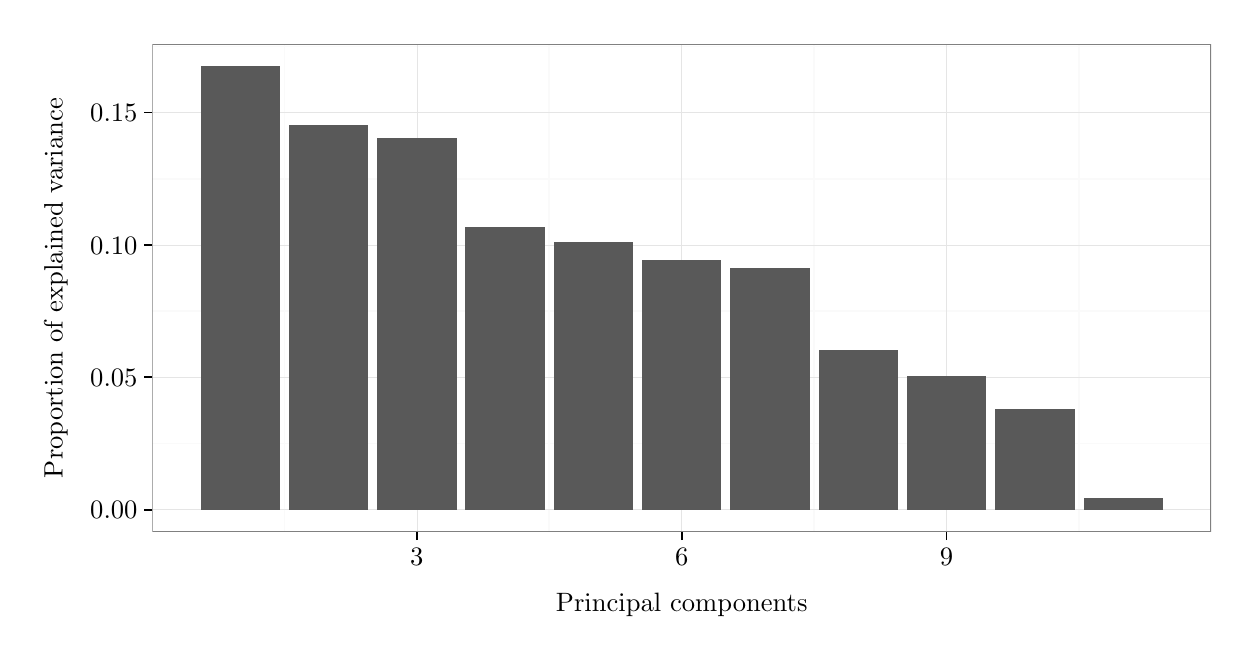
\begin{tikzpicture}[x=1pt,y=1pt]
\definecolor{fillColor}{RGB}{255,255,255}
\path[use as bounding box,fill=fillColor,fill opacity=0.00] (0,0) rectangle (433.62,216.81);
\begin{scope}
\path[clip] (  0.00,  0.00) rectangle (433.62,216.81);
\definecolor{drawColor}{RGB}{255,255,255}
\definecolor{fillColor}{RGB}{255,255,255}

\path[draw=drawColor,line width= 0.6pt,line join=round,line cap=round,fill=fillColor] (  0.00,  0.00) rectangle (433.62,216.81);
\end{scope}
\begin{scope}
\path[clip] ( 45.07, 34.62) rectangle (427.62,210.81);
\definecolor{fillColor}{RGB}{255,255,255}

\path[fill=fillColor] ( 45.07, 34.62) rectangle (427.62,210.81);
\definecolor{drawColor}{gray}{0.98}

\path[draw=drawColor,line width= 0.6pt,line join=round] ( 45.07, 66.54) --
	(427.62, 66.54);

\path[draw=drawColor,line width= 0.6pt,line join=round] ( 45.07,114.37) --
	(427.62,114.37);

\path[draw=drawColor,line width= 0.6pt,line join=round] ( 45.07,162.19) --
	(427.62,162.19);

\path[draw=drawColor,line width= 0.6pt,line join=round] ( 45.07,210.01) --
	(427.62,210.01);

\path[draw=drawColor,line width= 0.6pt,line join=round] ( 92.77, 34.62) --
	( 92.77,210.81);

\path[draw=drawColor,line width= 0.6pt,line join=round] (188.49, 34.62) --
	(188.49,210.81);

\path[draw=drawColor,line width= 0.6pt,line join=round] (284.21, 34.62) --
	(284.21,210.81);

\path[draw=drawColor,line width= 0.6pt,line join=round] (379.92, 34.62) --
	(379.92,210.81);
\definecolor{drawColor}{gray}{0.90}

\path[draw=drawColor,line width= 0.2pt,line join=round] ( 45.07, 42.63) --
	(427.62, 42.63);

\path[draw=drawColor,line width= 0.2pt,line join=round] ( 45.07, 90.46) --
	(427.62, 90.46);

\path[draw=drawColor,line width= 0.2pt,line join=round] ( 45.07,138.28) --
	(427.62,138.28);

\path[draw=drawColor,line width= 0.2pt,line join=round] ( 45.07,186.10) --
	(427.62,186.10);

\path[draw=drawColor,line width= 0.2pt,line join=round] (140.63, 34.62) --
	(140.63,210.81);

\path[draw=drawColor,line width= 0.2pt,line join=round] (236.35, 34.62) --
	(236.35,210.81);

\path[draw=drawColor,line width= 0.2pt,line join=round] (332.06, 34.62) --
	(332.06,210.81);
\definecolor{fillColor}{gray}{0.35}

\path[fill=fillColor] ( 62.46, 42.63) rectangle ( 91.18,202.80);

\path[fill=fillColor] ( 94.37, 42.63) rectangle (123.08,181.75);

\path[fill=fillColor] (126.27, 42.63) rectangle (154.99,176.77);

\path[fill=fillColor] (158.18, 42.63) rectangle (186.89,144.71);

\path[fill=fillColor] (190.08, 42.63) rectangle (218.80,139.32);

\path[fill=fillColor] (221.99, 42.63) rectangle (250.70,132.89);

\path[fill=fillColor] (253.90, 42.63) rectangle (282.61,129.93);

\path[fill=fillColor] (285.80, 42.63) rectangle (314.52,100.35);

\path[fill=fillColor] (317.71, 42.63) rectangle (346.42, 91.10);

\path[fill=fillColor] (349.61, 42.63) rectangle (378.33, 78.86);

\path[fill=fillColor] (381.52, 42.63) rectangle (410.23, 46.94);
\definecolor{drawColor}{gray}{0.50}

\path[draw=drawColor,line width= 0.6pt,line join=round,line cap=round] ( 45.07, 34.62) rectangle (427.62,210.81);
\end{scope}
\begin{scope}
\path[clip] (  0.00,  0.00) rectangle (433.62,216.81);
\definecolor{drawColor}{RGB}{0,0,0}

\node[text=drawColor,anchor=base east,inner sep=0pt, outer sep=0pt, scale=  0.96] at ( 39.67, 39.33) {0.00};

\node[text=drawColor,anchor=base east,inner sep=0pt, outer sep=0pt, scale=  0.96] at ( 39.67, 87.15) {0.05};

\node[text=drawColor,anchor=base east,inner sep=0pt, outer sep=0pt, scale=  0.96] at ( 39.67,134.97) {0.10};

\node[text=drawColor,anchor=base east,inner sep=0pt, outer sep=0pt, scale=  0.96] at ( 39.67,182.80) {0.15};
\end{scope}
\begin{scope}
\path[clip] (  0.00,  0.00) rectangle (433.62,216.81);
\definecolor{drawColor}{RGB}{0,0,0}

\path[draw=drawColor,line width= 0.6pt,line join=round] ( 42.07, 42.63) --
	( 45.07, 42.63);

\path[draw=drawColor,line width= 0.6pt,line join=round] ( 42.07, 90.46) --
	( 45.07, 90.46);

\path[draw=drawColor,line width= 0.6pt,line join=round] ( 42.07,138.28) --
	( 45.07,138.28);

\path[draw=drawColor,line width= 0.6pt,line join=round] ( 42.07,186.10) --
	( 45.07,186.10);
\end{scope}
\begin{scope}
\path[clip] (  0.00,  0.00) rectangle (433.62,216.81);
\definecolor{drawColor}{RGB}{0,0,0}

\path[draw=drawColor,line width= 0.6pt,line join=round] (140.63, 31.62) --
	(140.63, 34.62);

\path[draw=drawColor,line width= 0.6pt,line join=round] (236.35, 31.62) --
	(236.35, 34.62);

\path[draw=drawColor,line width= 0.6pt,line join=round] (332.06, 31.62) --
	(332.06, 34.62);
\end{scope}
\begin{scope}
\path[clip] (  0.00,  0.00) rectangle (433.62,216.81);
\definecolor{drawColor}{RGB}{0,0,0}

\node[text=drawColor,anchor=base,inner sep=0pt, outer sep=0pt, scale=  0.96] at (140.63, 22.61) {3};

\node[text=drawColor,anchor=base,inner sep=0pt, outer sep=0pt, scale=  0.96] at (236.35, 22.61) {6};

\node[text=drawColor,anchor=base,inner sep=0pt, outer sep=0pt, scale=  0.96] at (332.06, 22.61) {9};
\end{scope}
\begin{scope}
\path[clip] (  0.00,  0.00) rectangle (433.62,216.81);
\definecolor{drawColor}{RGB}{0,0,0}

\node[text=drawColor,anchor=base,inner sep=0pt, outer sep=0pt, scale=  0.96] at (236.35,  6.00) {Principal components};
\end{scope}
\begin{scope}
\path[clip] (  0.00,  0.00) rectangle (433.62,216.81);
\definecolor{drawColor}{RGB}{0,0,0}

\node[text=drawColor,rotate= 90.00,anchor=base,inner sep=0pt, outer sep=0pt, scale=  0.96] at ( 12.61,122.72) {Proportion of explained variance};
\end{scope}
\end{tikzpicture}

    \caption{PCA scree plot.}
    \label{fig:pca_screeplot}
\end{figure}

\begin{figure}[!p]
    \center
    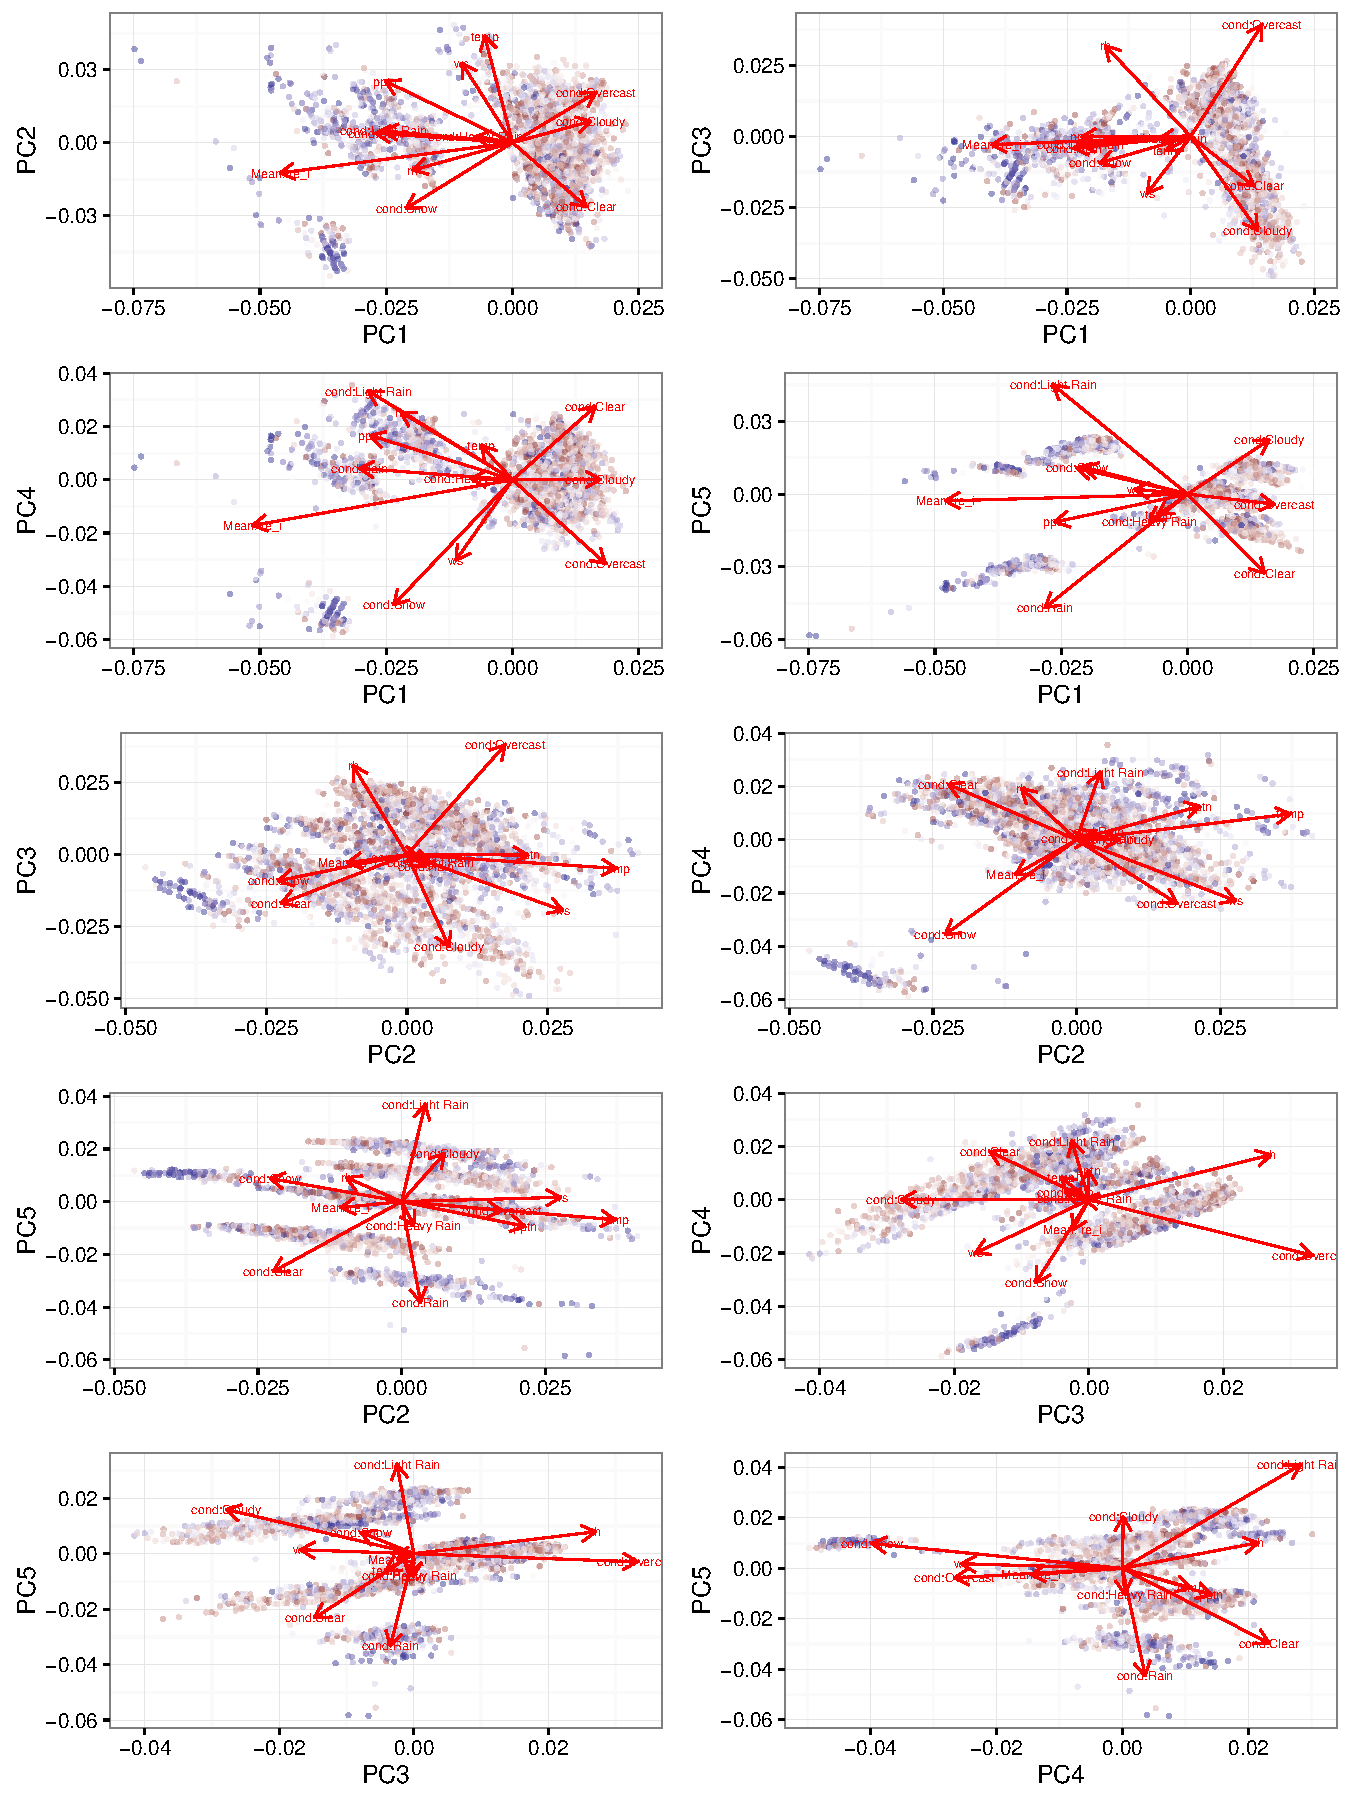
\includegraphics[width=\textwidth]{../plots/pca_loadings}
    \caption{PCA loadings for PC1--PC5.}
    \label{fig:pca_loadings}
\end{figure}
\clearpage

\subsection{Support vector machine}
In order to handle the original goal of presenting an prediction model for travel demand cf.\ \Cref{ch:objective}, a simple \emph{Support vector machine} (SVM) was trained. Since SVM is a supervised learning model, it should be able to re-project the weather data for the use of travel demand prediction to a larger degree than the PCA was able to.

For simplification the travel demand deviation was divided into 3 categories by the $^1/_3$ and $^2/_3$ quantiles of \gls{re_i}. The resulting tree groups was named Low ($\gls{re_i} < -5.5\%$), Normal ($-5.5\% <= \gls{re_i} < 4.9\%$) and High ($4.9\% <= \gls{re_i}$). The dataset is splitted in to a train and test dataset (first 80\% of data i used for training, the last 20\% for testing). The SVM is than trained to predict the demand category based on the training weather data as input (again discrete values are replaced with dummy variables), and tested on the test data set.

The results is shown in \Cref{fig:svm_prediction}, and it is seen that in all tree cases the model is able to predict unseen travel demand to the right group with $>40\%$ accuracy, compared to $\approx33\%$ of pure random classification. There are however significant errors, which cloud be an effect of travel demand deviation caused by other external factors than weather (e.g.\ events), or that the model can be improved further.

\begin{figure}[!ht]
    \center
    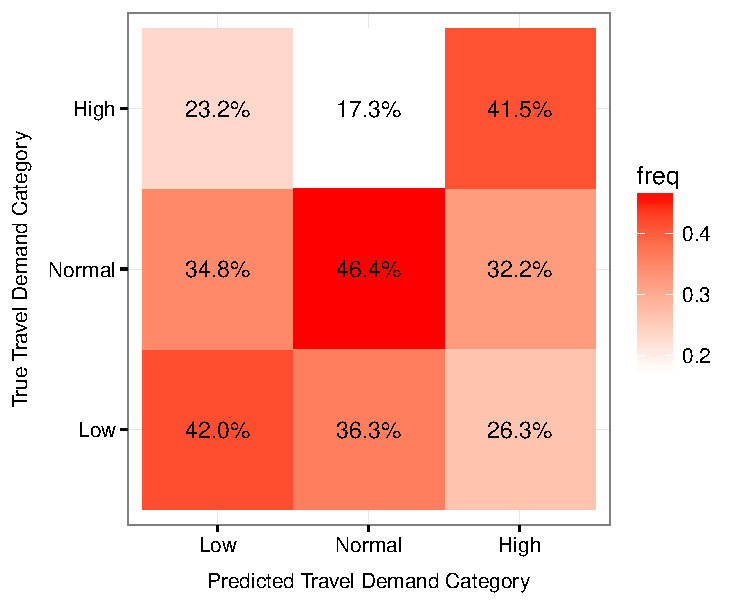
\includegraphics{../plots/svm_prediction}
    \caption{SVM prediction accuracy.}
    \label{fig:svm_prediction}
\end{figure}